\section{Mise en œuvre de la solution} 

La base de données étant un élément essentiel du projet, elle se devait d’être très générique. En effet, cette contrainte fait partie du cahier des charges. Elle doit pouvoir accueillir les données des capteurs déjà existants mais aussi des capteurs qui pourraient être ajoutés plus tard. Cette base doit pouvoir sauvegarder aussi bien les données des capteurs que leurs caractéristiques et les métadonnées.

Malgré l'importance de la modélisation de la base de données nous avons pris la décision de commencer par l'extraction des données des stations météo. Cela m'a permis de me familiariser avec les données issues des capteurs. Sur les conseils de mon maître de stage, j'ai réalisé un modèle de base de données assez simple et le plus évolutif possible, facile à comprendre, pour avoir une idée générale et on s’est réservé le droit de le modifier et de l’améliorer tant que cela soit possible. 

Simultanément, j’ai pu commencer à travailler sur le programme extracto-chargeur de données météo des stations se trouvant sur le site de Montoldre. Ainsi j’ai pu appréhender la notion de données sur les données en générale et les données météo en particuliers.  

 
Sur le site de Montoldre, deux stations météo avaient été installées. Valentin Mère, stagiaire sur le même projet basé sur le site de Montoldre s’était occupé de la partie acquisition de données comme par exemple installer et tester le bon fonctionnement des stations. Depuis le site d’IRSTEA Aubière, j‘avais accès aux données via le réseau Intranet d’IRSTEA. Une visite sur les lieux m’a permis de me rendre compte des dispositifs avec lesquelles je travaillais à distance.  

\subsection{Les stations météo du site de Montoldre} 

\subsubsection{Station météo Sencrop}

\begin{wrapfigure}{r}{.3\textwidth}
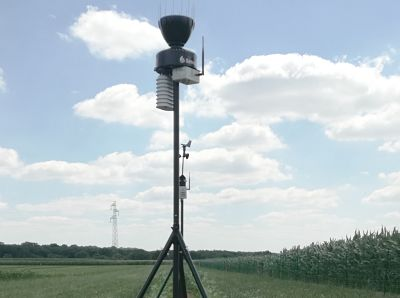
\includegraphics[width=4cm]{images/imageRang3.jpg}
\end{wrapfigure}
Sencrop est un ensemble de deux stations, un pluviomètre(raincrop) et un annémomètre (windcrop) produit par une société française basée à Lille et spécialisée dans la météo pour l’agriculture. La station Sencrop est dotée de capteurs qui enregistrent la pluviométrie, la température de l’air, l’hygrométrie, la vitesse et la direction du vent. Elle envoie ses données toutes les quinze minutes via une API et celles-ci peuvent être accessibles sur un smart phone, une tablette ou un ordinateur. Cette station a été installée au courant du mois de juin 2018. 

\subsubsection{Station météo Davis vantage Pro 2}

Installée en 2010, la station Davis est un produit du groupe CIMA TECHNOLOGIE FRANCE. Station sans fil, elle comprend une suite intégrée de capteurs météo et une console de visualisation des données, mesure. Elle mesure le vent (vitesse et direction), la pluviométrie, la température et l'humidité sous abri à ventilation naturelle, l'humidité intérieure et extérieure, pression barométrique. La portée radio en espace libre est de 300 m.


